\documentclass[oneside,10pt]{book}

\usepackage{cdtBook}
\usepackage{usecases}
\usepackage{requerimientos/requisitos}
\usepackage{amsmath}
\usepackage{amssymb}
\usepackage{booktabs}
\usepackage{hyperref}
\usepackage{enumerate}
\usepackage{mensajes/msg_style}
\usepackage{pdfpages} %Para cargar pdfs
\usepackage{estilos/estilos}
%\overfullrule=2cm

%\title{Análisis}
%\subtitle{}
%\author{Autores: \\Fernández Quiñones Isaac\\Huerta Martínez Jesús Manuel\\Pérez García José David}
%\organization{Escuela Superior de Cómputo, IPN}

%%%%%%%%%%%%%%%%%%%%%%%%%%%%%%%%%%%%%%%%%%%%%%%%%%%%%%%%%%%%%%%%
\begin{document}

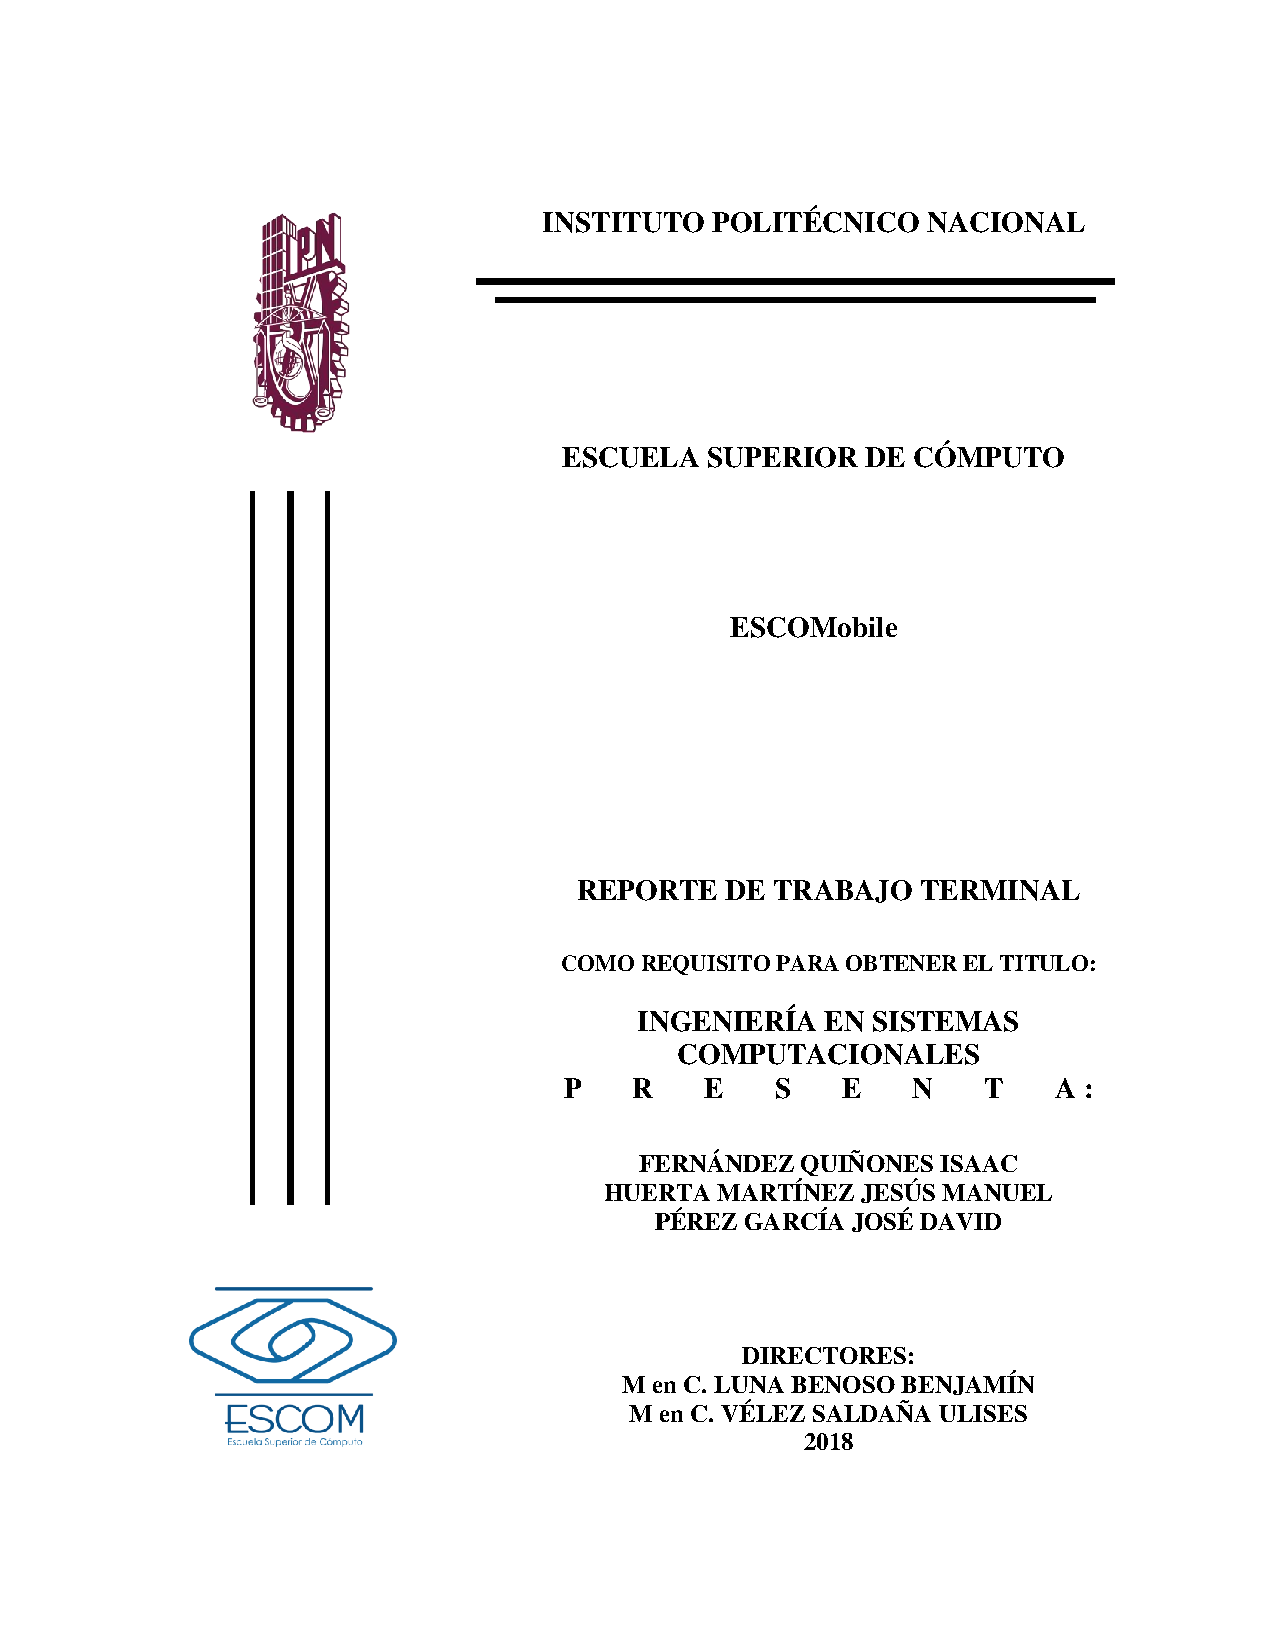
\includepdf[pages=1]{portada/posible_portada}

%\maketitle
%\thispagestyle{empty}
\frontmatter
\tableofcontents
\listoffigures
\listoftables
\mainmatter

%=========================================================
%                                                         INTRODUCCIÓN.
%=========================================================

\chapter{Introducción}

% Introducción.
\cfinput{intro/Introduccion_doctec}
% Justificación.
\cfinput{intro/Justificacion}
% Objetivos.
\cfinput{intro/Objetivos}
% Glosario.
\cfinput{marco_teorico/glosario}

%=========================================================
%                                                        ANTECEDENTES.
%=========================================================

\chapter{Planteamiento del proyecto}

% Marco teórico.
\cfinput{antecedentes/marco_teorico}
% Propuesta.
\cfinput{antecedentes/propuesta}
% Estado del arte.
\cfinput{antecedentes/estadoarte}
% Análisis de riesgos.
\cfinput{riesgos/analisisderiesgos}

%=========================================================
%                                                            REQUISITOS.
%=========================================================

\chapter{Requisitos de software}

% Requerimientos.
\cfinput{requerimientos/requisitos}	
% Tecnologías a usar.
\cfinput{requerimientos/tecnologias}

%=========================================================
%                                                     REGLAS DE NEGOCIO.
%=========================================================

\chapter{Modelo de Negocios}
\cfinput{reglas_negocio/reglas}

%=========================================================
%                                                         CASOS DE USO.
%=========================================================

% Descripción de casos.
\chapter{Descripción de los módulos del Sistema}
\cfinput{cu_temp/cu_temp}

% Modelado de casos.
\chapter{Modelo de Casos de Uso}
\noindent
Esta sección aborda el modelado de los casos de uso previamente descritos que conformarán la aplicación ESCOMobile. Aquí se detalla la información referente a cada Caso de Uso, sus características como, resumen, propósitos, entradas, salidas, etc., así como las trayectorias principal y alternativas que en los casos se contemplan. 

% Módulo de acceso. 
\cfinput{cu/EM-Acceso/CU01}
\cfinput{cu/EM-Acceso/CU02}
\cfinput{cu/EM-Acceso/CU03}
\cfinput{cu/EM-Acceso/CU04}
\cfinput{cu/EM-Acceso/CU05}
\cfinput{cu/EM-Acceso/CU06}

% Módulo de Mapa.
\cfinput{cu/EM-Mapa/CU01}
\cfinput{cu/EM-Mapa/CU02}

% Módulo de Alumno.
\cfinput{cu/EM-Alumno/CU1}
\cfinput{cu/EM-Alumno/CU1_1}

% Módulo de AlumnoBolsa.
\cfinput{cu/EM-AlumnoBolsa/CU1}
\cfinput{cu/EM-AlumnoBolsa/CU1_1}

% Módulo de AlumnoProfesor. 
\cfinput{cu/EM-AlumnoProfesor/CU1}
\cfinput{cu/EM-AlumnoProfesor/CU1_1}
\cfinput{cu/EM-AlumnoProfesor/CU1_1_1}
\cfinput{cu/EM-AlumnoProfesor/CU1_1_2}
\cfinput{cu/EM-AlumnoProfesor/CU1_1_3}
\cfinput{cu/EM-AlumnoProfesor/CU1_1_3_1}
\cfinput{cu/EM-AlumnoProfesor/CU1_1_4}

% Módulo de Pofesor.
\cfinput{cu/EM-Profesor/CU1}
\cfinput{cu/EM-Profesor/CU1_1}
\cfinput{cu/EM-Profesor/CU1_2}
\cfinput{cu/EM-Profesor/CU1_2_1}
\cfinput{cu/EM-Profesor/CU1_3}
\cfinput{cu/EM-Profesor/CU2}

% Módulo de Citas.
\cfinput{cu/EM-Citas/CU1}
\cfinput{cu/EM-Citas/CU1_1}
\cfinput{cu/EM-Citas/CU1_2}
\cfinput{cu/EM-Citas/CU1_2_1}
\cfinput{cu/EM-Citas/CU1_2_2}
\cfinput{cu/EM-Citas/CU1_3}
\cfinput{cu/EM-Citas/CU1_3_1}
\cfinput{cu/EM-Citas/CU1_4}
\cfinput{cu/EM-Citas/CU1_4_1}
\cfinput{cu/EM-Citas/CU2}

% Módulo de BolsaWeb.
\cfinput{cu/EM-BolsaWeb/CU1}
\cfinput{cu/EM-BolsaWeb/CU1-1}
\cfinput{cu/EM-BolsaWeb/CU1-2}
\cfinput{cu/EM-BolsaWeb/CU1-3}
\cfinput{cu/EM-BolsaWeb/CU3}
\cfinput{cu/EM-BolsaWeb/CU4}
\cfinput{cu/EM-BolsaWeb/CU4_1}
\cfinput{cu/EM-BolsaWeb/CU4_2}
\cfinput{cu/EM-BolsaWeb/CU4_3}

% Bolsa de trabajo Web. 
%\cfinput{cu/EM-BolsaWeb/CU1}
%\cfinput{cu/EM-BolsaWeb/CU1-1}
%\cfinput{cu/EM-BolsaWeb/CU1-2}
%  /\cfinput{cu/EM-BolsaWeb/CU1-3}
%\cfinput{cu/EM-BolsaWeb/CU1-4}
%\cfinput{cu/EM-BolsaWeb/CU2}
%\cfinput{cu/EM-BolsaWeb/CU3}
%\cfinput{cu/EM-BolsaWeb/CU4}
%\cfinput{cu/EM-BolsaWeb/CU4_1}
%\cfinput{cu/EM-BolsaWeb/CU4_2}
%\cfinput{cu/EM-BolsaWeb/CU4_3}

%=========================================================
%                                                    MODELO DE INTERACCION
%=========================================================

\chapter{Modelo de la Interacción}

\noindent
En este apartado se muestran las diferentes pantallas que componen a la aplicación ESCOMobile,
la forma en que éstas se estructuran y la descripción de las diferentes secciones que las componen.
La información que se puede consultar en la descripción incluye: objetivo, descripción del diseño, 
una imagen que ilustra el diseño descrito, las entradas requeridas (de ser el caso) y las salidas
generadas y mostradas dentro de la propia pantalla, así como los comandos y mensaje con las que
éstas pueden llegar a contar.

\noindent
\newline
A continuación, se muestra la descripción de cada una de las pantallas que forman ESCOMobile,
en el mismo orden del cual se describieron los casos de uso.

% Pantallas.
\cfinput{Pantallas/Acceso/UI_Acceso}
\cfinput{Pantallas/Mapa/UI_Mapa}
\cfinput{Pantallas/Alumno/UI_Alumno}
\cfinput{Pantallas/AlumnoBolsa/UI_AlumnoBolsa}
\cfinput{Pantallas/AlumnoProfesor/UI_AlumnoProfesor}
\cfinput{Pantallas/Profesor/UI_Profesor}
\cfinput{Pantallas/Citas/UI_Citas}
\cfinput{Pantallas/BolsaWeb/UI_WebBolsa}



%=========================================================
%                                                                MENSAJES.
%=========================================================

\chapter{Modelo de mensajes}
\cfinput{mensajes/mensajes}

%=========================================================
%                                                     DOMINIO DEL PROBLEMA.
%=========================================================

\chapter{Modelo del Dominio del problema}

\noindent
En esta sección se define la estructura que tiene el sistema, los componentes que hacen que
funcione y que hace posible que los casos de uso puedan integrarse. Se muestran también los
diagramas de clases en los cuales el desarrollo de la aplicación está basado y el diagrama de 
base de datos que interactúa con la misma para brindar el servicio final. 
A continuación, se presentan cada uno de estos apartados.

%  Arquitectura.
\cfinput{dominio/arquitectura}
%  Diagramas de clases..
\cfinput{dominio/clases}
%  Base de datos.
\cfinput{dominio/baseDatos}

%=========================================================
%                                                              BIBLIOGRAFIA.
%=========================================================

\cfinput{bibliografia/bibliografia}

% FIN DEL DOCUMENTO.
\end{document}
